\subsection{Challenge 1: Requirements Formalization}

While model-based approaches, supported by formal reasoning tools, can be used to verify if implementation models meet requirements, the process of formalizing the requirements from the natural language documents is often a laborious process. Although, natural language (NL) is the practical choice for capturing requirements, formal methods are necessary to rigorously verify them. For complex systems, the process of formalizing requirements becomes a non-trivial activity. The challenge arises from both the ambiguity and implicit contextual knowledge in the NL statements. While the process of formalization implicity takes care of the ambiguity, precisely identifying the context of the requirement is a painful process. By contextual nature of requirements, we mean the specific state of the system in which the requirements need to hold; in formal terms it is the antecedent or precondition in a formal statement. While well known specification patterns focus on recapturing the NL statements to formal notations, they do not help to address the challenge of identifying the context of the requirements. To partially address this concern in domains such as safety critical systems, the formalized requirements are verified with respect to a model of the system. When the context is not sufficiently captured in the formalized requirement, tools such as model checkers return counterexamples to help engineers discover the needed contextual information. However, this counterexample directed context exploration is a very time-consuming task, especially for certain types of requirements.

When formalizing the requirements of the GPCA, we found two groups of requirements whose context was particularly challenging to identify. The first set of requirements were those that describe the behaviour of the system under under normal working conditions. For example, one requirement states\footnote{\scriptsize{We intensionally simplified this requirement such that it illustrates the problem. However, the original requirement had more conditions associated with it.}} that,

\begin{quotation}
\emph{``When the patient requests a bolus, the system shall deliver an the drug at flow rate equal to $patient\_flow\_rate$ ''}
\end{quotation}

When we initially tried to formalize and verify the requirement, the model checker repeatedly returned counter examples. A careful examination of the counter examples revealed that there were certain conditions in the system that prevented the patient bolus infusion from occurring and hence the requirement was not satisfied in that context. These conditions were actually safety features of the system to prevent hazards that were documented as ``alarm requirements" in another section in the requirements document.  Unfortunately, traceability between such requirements was neither available nor establishing and maintaining then was practically straightforward, due to the numerous requirements and the orthogonality/exclusivity between the behaviours the requirements capture.

The second group of requirements that were difficult to formalize were those that were mutually exclusive, but had a certain inherent priority among them. In the GPCA, the alarm requirements capture the system's responses to exceptional conditions. There were 18 exceptional conditions identified for the GPCA, each with its own set of desired system responses depending upon the severity level of that condition. For example, the system responds to a high severity condition such as an empty drug reservoir by raising an audio alarm, displaying error message, and stopping infusion. On the other hand, when the system has been idle for a long time and a low severity level alarm is triggered, the system only displays an appropriate message. One of the problems we encountered was formalizing the requirement in such a way that verifies their effect independently. For instance, to verify a lower priority condition requirement we had to systematically ensure all the higher priority ones did not occur. The problem was that there was no explicit priority specified in the requirements document and we had to infer the priority based on the system responses. Unfortunately, there was no guidance or patterns to help systematically organize and formalize such requirements for verification. On the contrary, the GPCA model that implements the requirement had a specific prioritization mechanism (that we believe is a design decision of the developer implementing the requirements). Formalizing and verifying each alarm condition requirements independently without including the design decisions of the model was a big challenge. We realized that root cause of this problem is the undisciplined organization of the requirements statements within the document.

\subsubsection {Approach: Structuring Requirements}

To systematically identify the context of each requirement and its dependencies with other requirements, we hierarchically restructured the GPCA requirement document as shown in Figure~\ref{fig:gpca-requirements}, that not only simplified the formalization process also helped understand the system in a conceptually clear way. The system behaviors of most control systems are typically captured by grouping them in terms of \emph{modes} - a logical way to describe a set of system behaviours. In a complex system, there could be many modes that could either be mutually exclusive (only one mode can be active at a time) or orthogonal (multiple modes can be active at a time). By grouping the modes based on their common and exclusive behaviours as well as their interactions, we hierarchically organized them that helped systematically documenting, formalizing and verifying the requirements.

 \begin{figure}[h!]
    \centering
    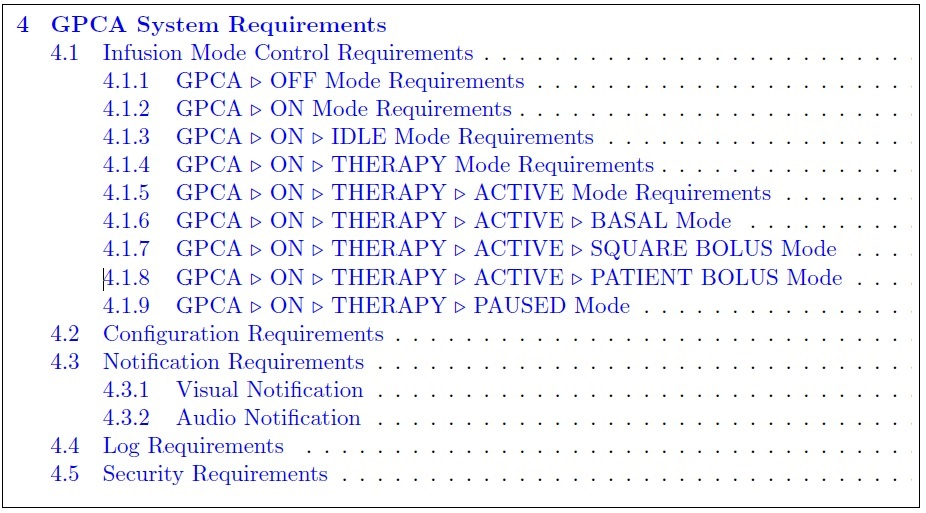
\includegraphics[width=\columnwidth]{images/structuring.jpg}
    \caption{GPCA System Requirements Structuring}
    \label{fig:gpca-requirements}
 \end{figure}

In the GPCA, there were three main orthogonal groups of modes - infusion, configuration and notification modes. Within each orthogonal group, there were a set of modes that were mutually exclusive to each other such as basal, intermittent and patient bolus modes within infusion mode group. Similarly, the notification group had 18 requirements that we further categorized based on its severity level (Levels 4 to 1). When we analysed the requirements, we understood that there were many requirements that were common to the exclusive modes among an orthogonal group, as well as requirements that were common to all the three orthogonal mode groups. We leveraged this pattern of modal requirements to organize requirement statements within the document in an hierarchial fashion. In this structuring, at the top most level we placed requirements that were common to the entire system. At the next level, we placed the mode groups that were orthogonal to each other. Within each orthogonal mode group, we again followed the hierarchical structure to organize their requirements. For clarity purposes, within a mode group we grouped requirements hierarchically based on their behaviours and named it as a new mode (although it was not explicitly mentioned by the stakeholders). For example, we placed all the requirements that were common among the basal and boluses infusions in a parent mode called \emph{Therapy} mode and made the basal and bolus its child modes with its own set of special requirements. For additional clarity on understanding the mutual exclusivity among modal behaviours, we documented requirements using a tabular notation. An example of the tabular format we used for the notification requirements is shown in Figure~\ref{fig:gpca-alarm}. Although we came across a couple of requirements that had minor variations to be grouped, this structuring helped identify those differences and we were able to clearly negotiate with our domain experts on appropriately categorizing them.

 \begin{figure}[h!]
    \centering
    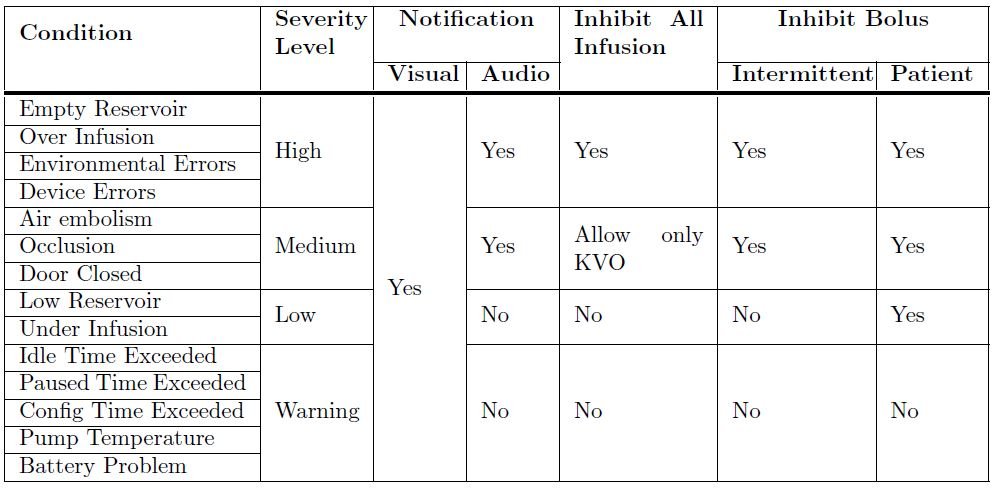
\includegraphics[width=\columnwidth]{images/alarm.jpg}
    \caption{Notification Requirements Table}
    \label{fig:gpca-alarm}
 \end{figure}


This structuring greatly helped in systematically determining the context of each requirement while formalizing it. It provided enough information about the orthogonality and exclusivity among the modes. For instance, by examining the requirements hierarchically from the top level, we were able to precisely identify and formalize the context of the patient bolus infusion requirement and the notification requirements that were discussed in Section 3.1. While such hierarchical structuring is common among modeling community, it has not been widely used to document requirements in the requirements engineering community. We believe that using such a strategy not only helps reducing the effort for formalizing requirements, but also provides the intellectual clarity to understand the system behaviours.

